\section{BFS}

% \subsection{Практика}
% \begin{enumerate}

%   \item
%     Даны три бочки на 10, 7 и 4 литра. 7- и 4-литровые бочки
%     заполнены водой.  Разрешается переливать воду между бочками, 
%     либо пока одна бочка не заполнится полностью, либо пока 
%     другая не опустеет. Проверить, можно ли получить 2 литра в любой из бочек. 
%     Если возможно, найти минимальное необходимое число переливаний.  
%     Как решить аналогичную задачу, если емкости бочек $a$, $b$
%     и $c$ ($a, b, c \in \mathbb{N}, \, a \leq b \leq c$), а бочки с ёмкостями $a$ и $b$ заполнены
%     водой? Время: $\O(a \cdot b)$.

%   \item
%     Найти количество путей (необязательно простых) в графе за $\O(V^3 \log{k})$
%     \begin{enumerate}
%     	\item между всеми парами вершин длины ровно $k$.
%     	\item между парой вершин длины $\le k$.
%     \end{enumerate}

%   \item
% 	  Найти в орграфе все вершины, через которые проходит какой-нибудь кратчайший путь $a \leadsto b$. $\O(V + E)$.

%   \item
%     Пусть в графе есть ребра веса $0$ и $1$. Придумайте, как найти
%     кратчайшее расстояние от вершины $s$ до остальных за $\O(V + E)$.

%   \item
%     Пусть в графе все ребра имеют целый вес из $[1, k]$. Придумайте, как найти
%     кратчайшее расстояние от вершины $s$ до остальных.
%     \begin{enumerate}
%       \item $k = 2$, $\O(V + E)$
%       \item $k$ --- произвольное, $\O(V + kE)$.
%       \item $k$ --- произвольное, $\O(k V + E)$.
%       \item $k$ --- произвольное, $\O(E \log{k})$.
%     \end{enumerate}

%   \item
%     Дан орграф с положительными весами на ребрах. Найти кратчайший путь, проходящий по всем $k$ выделенным вершинам. 
%     Время $\O(2^k E \log{(2^k V)})$.

% \subsection*{Дополнительные задачи}

%   \item
% 	Пусть длина пути определяется как сумма весов всех ребер по модулю $n$.
% 	Найти кратчайший путь за $\O((V+E)n)$.

%   \item
%     В стране $n$ аэропортов. Самолет может сделать перелет 
%     из аэропорта $i$ в аэропорт $j$, израсходовав $w_{ij} > 0$ горючего.
%     При этом $w_{ij}$ может отличаться от $w_{ji}$, и $w_{ii} = 0$.
% 	Требуется найти минимальный размер бака, позволяющий добраться
% 	самолету из любого города в любой, возможно с дозаправками.
% 	Решить за $\O(n^2)$.

%   \item
%     \begin{enumerate}
%       \item $k$-$2k$-bfs, веса вещественные.
%       \item $k$-$2k$-bfs, веса целые, хотим делать только целочисленные операции.
%     \end{enumerate}

%   \item
% 	Даны две параллельных прямых (река). В реке есть $n$ островов (точек). Мы хотим провести по
% 	реке корабль, представляющий собой открытый круг радиуса $R$, так, чтобы он не задел ни одного острова.
% 	Найти максимальный $R$, при котором это еще возможно, за $\O(n^2)$.

% \end{enumerate}

% \pagebreak

\subsection{Домашнее задание}
\begin{enumerate}
  \item
    Дан взвешенный орграф с положительными весами и вершина $s$.
    Нужно для каждой вершины $v$ найти число кратчайших путей из $s$ в $v$ по модулю $p$. $\O(E \log V)$.
    \begin{solution}
      Воспользуемся алгоритмом Дейкстры для решения данной задачи. Модернизируем только этот алгоритм в одном месте -- будем хранить для каждой вершины еще и счетчик (количество кратчайших путей до этой вершины, инициализируем до первой вершины -- 1, до остальных -- 0) и когда мы вытащили очередную вершину из очереди и смотрим, в какие вершины идут из нее ребра, то, если известное кратчайшее расстояние для этой вершины совпадает с [расстояние до текущей плюс вес ребра], то увеличиваем счетчик на значение счетчика в текущей вершине и берем модуль по $p$; если известное кратчайшее расстояние для этой вершины больше, чем [расстояние до текущей плюс вес ребра], то обновляем значение кратчайшего расстояния и делаем счетчик равным значению счетчика для текущей вершины; в противном случае ничего не делаем, продолжаем алгоритм.

      Корректность данного алгоритма опирается на корректность алгоритма Дейкстры, который не учитывает количество минимальных путей, и если он встречается с ситуацией, когда для какой-то вершины известное для нее кратчайшее расстояние совпадает с расстоянием до предыдущей плюс ребро, то ничего не происходит, он просто не обновляет значение кратчайшего расстояния для данной вершины. Модернизация алгоритма Дейкстры в виде добавления счетчика кратчайших путей по сути добавляет возможность отслеживать такие ситуации. Причем это работает корректно, ведь, если расстояние до следующей совпадает с расстоянием до текущей плюс соединяющее ребро, то счетчик увеличивается на значение счетчика текущей вершины, если то же самое расстояние оказывается большим, то счетчик обновляется до значения счетчика текущей вершины, а в противном случае, когда расстояние до следующей меньше, чем расстояние до текущей плюс ребро, счетчик никак не изменяется.

      Асимптотика данного алгоритма совпадает с асимптотикой алгоритма Дейкстры, потому что по сути добавляется всего лишь одна проверка, которая работает за $\O(1)$, а Дейкстра на $d$-куче работает за $\O(E \log V)$.
    \end{solution}

  \item
    В орграфе есть бесплатные и $K$ типов платных ребер. Передвижение
    по любому ребру стоит $0$, но, чтобы двигаться по платному ребру
    типа $x$, необходимо иметь пропуск того же типа. В любой момент
    времени можно иметь не более одного пропуска, однако в любой
    вершине есть возможность купить пропуск любого типа за $A$ и
    продать пропуск любого типа за $B$ ($0 < B < A$, цены одинаковы
    во всех вершинах). Найдите самый дешевый способ добраться из вершины
    $s$ до вершины $t$ за $\O(K (V + E))$.

  \item
    Дан ориентированный граф с выделенными вершинами $s$ и $t$. Перемещение по любому ребру занимает 1 единицу времени.
    В начальный момент времени мы стоим в вершине $s$, и во все ребра с постоянной скоростью $L$ начинает поступать вода.
    У каждого ребра $e$ есть емкость $C_e$ --- минимальное количество воды в этом ребре, при котором по нему больше
    нельзя двигаться (мы должны закончить движение по ребру не позднее момента достижения его емкости). Найдите
    максимальное $L$, при котором все еще существует возможность добраться от $s$ до $t$ за $\O((V + E)\log{C_{\max}})$.

  \item
    Постройте матрицу $n \times n$, состоящую из клеток-стенок и пустых клеток,
    на которой при запуске \texttt{BFS} из какой-то клетки максимальный
    размер очереди будет $\omega(n)$. Ходить можно между клетками, смежными по стороне.

  \item
    Попробуем научить алгоритм Дейкстры работать на графах с отрицательными весами: вынимаем из кучи вершину $v$
    с минимальным расстоянием и релаксируем все ребра из $v$. При этом вершины, до которых улучшилось расстояние,
    добавляются в кучу (или делается \texttt{DecreaseKey}, если вершина уже там).
    \begin{enumerate}
      \item Покажите, что этот алгоритм корректно вычисляет кратчайшие пути, если нет циклов отрицательного веса.
      \begin{solution}
        Циклов отрицательного веса действительно быть не должно, чтобы алгоритм продолжал быть корректным, потому что если есть отрицательный цикл, то, войдя в него, Дейкстра будет бесконечно крутиться в нем и не выйдет никогда. Если же циклов отрицательного веса нет, то даже если в графе есть ребра с отрицательными весами, то Дейкстра будет корректно вычислять кратчайшие пути, но только будет делать это медленнее (потому что одну и ту же вершину Дейкстра может положить в очередь больше, чем один раз). Проще всего показать этот факт на следующем примере:
        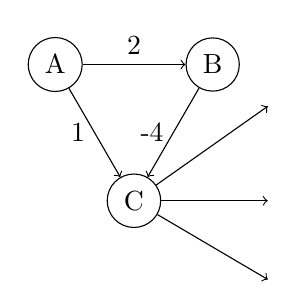
\begin{tikzpicture}
          \node[circle,draw] (A) at (0,0) {A};
          \node[circle,draw] (B) at (2,0) {B};
          \node[circle,draw] (C) at (1,-1.73) {C};
          
          \draw[->] (A) -- node[above] {2} (B);
          \draw[->] (A) -- node[left] {1} (C);
          \draw[->] (B) -- node[left] {-4} (C);
          \draw[->] (C) -- (2.7,-1.73);
          \draw[->] (C) -- (2.7,-2.73);
          \draw[->] (C) -- (2.7,-0.53);
        \end{tikzpicture}

        Мы изначально достаем вершину А и просчитываем кратчайшие расстояния до В (2) и С (1). Дальше достаем С, потому что у нее кратчайшее расстояние. Соответственно, для С мы релаксируем какие-то исходящие из нее ребра, просчитываем для каких-то других вершин кратчайшие расстояния, а потом в какой-то момент мы достаем вершину В и обновляем кратчайшее растояние до С, поэтому С снова кладется в очередь и после этого нужно заново релаксировать ее ребра. По сути работает тот же самый алгоритм Дейкстры, просто отрицательные ребра могут вот в таком ключе сильно замедлять его работу, никак не влияя на корректность его работы.
      \end{solution}
      \item Придумайте пример без циклов отрицательного веса, на котором время работы экспоненциально.
      \begin{solution}
        Можно составить конструкцию из треугольников следующим образом:

        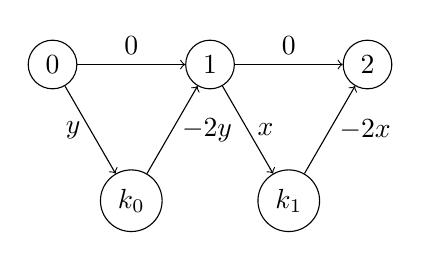
\begin{tikzpicture}
          \node[circle,draw] (A) at (0,0) {0};
          \node[circle,draw] (B) at (2,0) {1};
          \node[circle,draw] (C) at (1,-1.73) {$k_0$};
          \node[circle,draw] (D) at (4,0) {2};
          \node[circle,draw] (E) at (3,-1.73) {$k_1$};
          
          \draw[->] (A) -- node[above] {0} (B);
          \draw[->] (A) -- node[left] {$y$} (C);
          \draw[->] (C) -- node[right] {$-2y$} (B);
          \draw[->] (B) -- node[above] {0} (D);
          \draw[->] (B) -- node[right] {$x$} (E);
          \draw[->] (E) -- node[right] {$-2x$} (D);
        \end{tikzpicture}
        \hspace{1cm}
        \ldots
        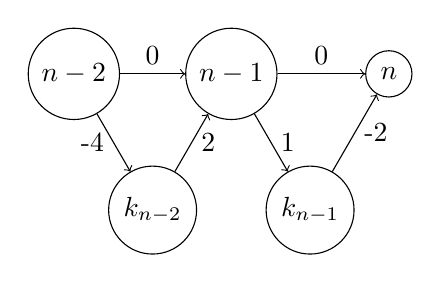
\begin{tikzpicture}
          \node[circle,draw] (A) at (0,0) {$n-2$};
          \node[circle,draw] (B) at (2,0) {$n-1$};
          \node[circle,draw] (C) at (1,-1.73) {$k_{n-2}$};
          \node[circle,draw] (D) at (4,0) {$n$};
          \node[circle,draw] (E) at (3,-1.73) {$k_{n-1}$};
          
          \draw[->] (A) -- node[above] {0} (B);
          \draw[->] (A) -- node[left] {-4} (C);
          \draw[->] (C) -- node[right] {2} (B);
          \draw[->] (B) -- node[above] {0} (D);
          \draw[->] (B) -- node[right] {1} (E);
          \draw[->] (E) -- node[right] {-2} (D);
        \end{tikzpicture}

        В таком случае понятно, что будет экспоненциальное время работы алгоритма, потому что он дойдет до самого конца (вершина $n$) по нулевым ребрам, потом будет вытаскивать из очереди нижние вершины справа налево и перепросчитывать свои результаты снова и снова, потому что отрицательное ребро каждый раз изменяет значение кратчайшего пути, что в свою очередь снова добавляет очередную вершину в очередь для повторной обработки. Количество перерасчетов в таком случае будет экспоненциально.
      \end{solution}
    \end{enumerate}

% \subsection*{Дополнительные задачи}

%   \item
%     Модифицируем условия задачи про бочки: есть $n$ бочек, $i$-я бочка имеет
%     объем $v_i$ ($v_i > 0$) и в начальный момент содержит $c_i$ воды
%     ($0 \le c_i \le v_i$). Операция переливания определена как в задаче из практики.
%     Придумайте такие $n$ и вещественные $v_i$, $c_i$, чтобы соответствующий граф
%     состояний, достижимых с помощью переливаний из начального, получился бесконечным.  

\end{enumerate}
